%!TEX root=../ctl-phd-thesis.tex

\section{Abstract}
Predicting the rate of nonfacilitated permeation of solutes across lipid bilayers is important to drug design, toxicology, and signaling. These rates can be estimated using molecular dynamics simulations combined with the inhomogeneous solubility-diffusion model, which requires calculation of the potential of mean force and position-dependent diffusivity of the solute along the transmembrane axis. In this paper, we assess the efficiency and accuracy of several methods for the calculation of the permeability of a model DMPC bilayer to urea, benzoic acid, and codeine. We compare umbrella sampling, replica exchange umbrella sampling, adaptive biasing forces, and multiple-walker adaptive biasing forces for the calculation of the transmembrane PMF. No definitive advantage for any of these methods in their ability to predict the permeability coefficient \perm was found, provided that a sufficiently long equilibration is performed. For diffusivities, a Bayesian inference method was compared to a Generalized Langevin method, both being sensitive to chosen parameters and the slow relaxation of membrane defects. Agreement within 1.5 log units of the computed \perm with experiment is found for all permeants and methods.  Remaining discrepancies can likely be attributed to limitations of the force field as well as slowly relaxing collective movements within the lipid environment.  Numerical calculations based on model profiles show that \perm can be reliably estimated from only a few data points, leading to recommendations for calculating \perm from simulations.


\section{Introduction}
\par Cells are the basic unit of life. An essential feature of cells is their encapsulating phospholipid membrane. Due to the hydrophobic effect~\cite{Tanford1979,Tanford1973}, individual phospholipids do not diffuse and tumble randomly.  Instead they form a bilayer structure with polar phosphate head groups on each side, facing the bulk solvent, with the apolar lipid tails forming a hydrophobic slab in between. This densely packed structure serves two primary purposes: (1) to contain and protect cellular machinery from the harsh external environment, and (2) to maintain ionic gradients to later harvest as energy. Lipid bilayers are an effective barrier to passive diffusion of ions and hydrophilic small molecules, such as carbohydrates, but many molecules can permeate bilayers through passive diffusion at rates that depend on bilayer composition and properties of the permeating solute. The semi-permeable nature of the membrane results in an effective ``selectivity,'' where small apolar compounds can cross the membrane at appreciable rates. In contrast to transmembrane ion channels and transporters that are carefully controlled by the cell, passive selectivity is not actively regulated, but instead arises intrinsically from the forces and fluctuations present across the membrane environment. Despite the enormous importance of passive permeability to basic cell function, a detailed mechanistic understanding of this phenomenon has yet to be achieved.

\par Estimation of passive permeation rates is of key importance, primarily for the delivery of candidate drugs to intracellular targets, as well as for later excretion of metabolites. For example, in 1991, $\sim$40\% of all attrition of drug candidates was related to adverse pharmacokinetic (PK) and bioavailability results~\cite{Kola2004}. PK attrition rates have since been reduced to about 10\% ~\cite{Tsaioun2009} primarily by high-throughput experimental measures of permeability such as the parallel artificial membrane permeability assay (PAMPA)~\cite{Kansy1998,Avdeef2005} and the cell-based CaCo-2 assay~\cite{Artursson2001,VanBreemen2005}. Although these empirical methods have become a mainstay in industry, they provide little to no insight into the biophysics of membrane permeation. To gain rational insight, assay results can be used to inform linear response models such as the quantitative structure permeability relationship (QSPR)~\cite{Hansch1972,Hansch1969}. Due to the nature of training models, QSPR exhibits mediocre predictive performance when compared across a broad range of experimental test sets~\cite{Stouch2003,Swift2013}. Despite advances in these technologies, neither experimental nor QSPR methods provide detailed atomistic insight into the permeation process.

\par To gain atomistic insight into the passive permeability process, physics-based methods, such as molecular dynamics (MD), have become increasingly popular. While the application of MD to passive permeability is alluring, broad adoption of the method is limited by several major outstanding challenges. First, there is much debate on the ability of current force fields to reproduce system thermodynamics and kinetics correctly~\cite{Paloncyova2014,Wang2015,Vitalini2015}. Second, the computational and human time burden is large; calculating the permeability of individual compounds can require thousands of CPU-years and months of work by an experienced researcher. Thus, in order to bring MD-based methods for passive permeability into broad practice, systematic studies addressing force field accuracy and computational efficiency of potential methods are warranted. Given the plethora of new experimental results, compound permeability is an ideal benchmark system for both computational free-energy and kinetics calculations that exist.

\par Passive membrane permeability has traditionally been studied using the homogeneous solubility-diffusivity model~\cite{Finkelstein1968}. Later work incorporating the heterogeneous nature of lipid bilayers led to the development of the inhomogeneous solubility-diffusion model~\cite{Diamond1974,Marrink1994}. The inhomogeneous solubility model is derived from the steady-state flux and assumes equilibrium across the membrane. Mathematically the potential of mean force (PMF), $W$($z$), and local diffusivity coefficient, $D$($z$), are related to the resistivity, $R$, and permeability, $P$, via the equation

\begin{equation}
R = \frac{1}{P} = \int_{z_1}^{z_2} \frac{\exp[\beta W(z)]}{D(z)}dz,
\label{eq:solubility-diffusion}
\end{equation}

where $\beta$ is the thermodynamic beta ($\beta=1/k_{B}T$), and $z$ is a collective variable describing the relative position of the solute along the transmembrane axis. The integration bounds, $z_1$ and $z_2$, are points along this axis on opposing sides of the membrane.
Both $W$($z$) and $D$($z$) can be estimated from MD simulations, provided that all $z$'s are well sampled.
Due to the nature of Boltzmann sampling, conventional MD is not ideal for sampling rare transition states. In order to obtain sufficient sampling of transition states, various importance sampling techniques have been developed. Some examples include umbrella sampling (US)~\cite{Torrie1977}, adaptive biasing force (ABF)~\cite{Rodriguez-Gomez2004,Darve2001,Darve2008a,Wei2011}, metadynamics~\cite{Laio2002}, and the Wang--Landau algorithm~\cite{Wang2001}. In general, many methods can be implemented with multiple replicas (RE) or walkers (MW) to further enhance sampling~\cite{Swendsen1986a}.
\par MD simulations have long been applied to study the mechanisms and rates of permeability; for a review please refer to Ref. \citenum{Xiang2006}. Many works have used various forms of US ~\cite{Wilson1996,Grossfield2002,Ulander2003a,Bemporad2004,MacCallum2007,Johansson2008,MacCallum2008,Bauer2011,Tejwani2011,MacCallum2011,Paloncyova2012,Swift2013,Riahi2014,Carpenter2014,Issack2015}, adaptive biasing force ~\cite{Bemporad2005,Comer2014a}, metadynamics~\cite{Ghaemi2012}, and kinetic master equations~\cite{Parisio2013}. Passive membrane permeability can also be calculated without the use of the solubility-diffusion equation via methods such as milestoning or directional milestoning~\cite{Kirmizialtin2011,Vanden-Eijnden2008,Majek2010,Bello-Rivas2015}. For example, milestoning has been used to determine the permeability of water as well as blocked tryptophan~\cite{Cardenas2012,Cardenas2014}.

\par While the aforementioned studies have examined the membrane permeability of individual solutes, there has not yet been a systematic examination of what the most effective method is for calculating $W$($z$) and $D$($z$). In particular, accurate calculations of $W$($z$) are difficult because of slowly converging orthogonal degrees of freedom, namely those related to membrane distortion and relaxation~\cite{Neale2011,Neale2014}. Umbrella sampling (US) is the canonical methodological approach, in which the solute is restrained at regular intervals along $z$. The effect of the restraints are analytically removed from the probability distributions calculated from the US simulations. These distributions are then combined into a single PMF covering the complete interval of the coordinate, employing a post-treatment analysis, e.g., the weighted histogram analysis method.  Replica-exchange US improves the sampling ergodicity of US simulations by attempting periodic exchanges between neighboring replicas. Conversely, the adaptive biasing force (ABF) algorithm adjusts the biasing force over time to sample the coordinate uniformly, whereas multiple walker ABF (MW-ABF) extends this further by spawning additional concurrent simulations in poorly explored regions of the coordinate.

\par In the present work, we systematically compare four methods: US, REUS, ABF, and MW-ABF, by calculating the permeability of urea, benzoic acid and codeine through a DMPC bilayer.


\section{Results and Discussion}
Below, we report the membrane permeability coefficients (\perm) of urea, benzoic acid, and codeine computed with four different methods, namely, US, REUS, ABF and MW-ABF.  We also present a detailed analysis of two methods for the computation of diffusivity, namely, a Bayesian inference method and a Generalized Langevin method. While we did not test metadynamics, another common free-energy method, it has recently been favorably compared with US for water-membrane partitioning, nonetheless while suffering the same shortcomings~\cite{Bochicchio2015}.  Initial states, i.e., positions of the permeant within the bilayer, were generated using 100-ns steered MD simulations~\cite{Izrailev1997,Sotomayor2007} in which the permeant is pulled from one side of the membrane to the other (see Methods).


The three permeants studied here, shown in Fig.\ref{fig:permeants}, are chosen for their diverse chemical properties:
their molecular weights range from 60\,g/mol (urea) to 299\,g/mol (codeine);
their hydrophilicity, as measured by the octanol:water partition coefficient, differs by over two orders of magnitude;
and most importantly, the experimentally determined \perm of the three permeants span five orders of magnitude (Table\,1), making them a relatively robust test set for \perm calculation via different methods. Of the three permeants, benzoic acid is the only permeant that exhibits a formal charge at pH=7. Nonetheless, only its neutral form is considered in our calculation. This treatment is consistent with the corresponding experimental protocol~\cite{Walter1984}, where fluxes at several pH values are measured to determine the `intrinsic permeability' corresponding to the un-ionized form of a given molecule. The underlying assumption of such a protocol, i.e., only the non-ionized form of benzoic acid contributes significantly to \perm, has been confirmed experimentally~\cite{Walter1984}.

\begin{figure}[htbp]
\begin{center}
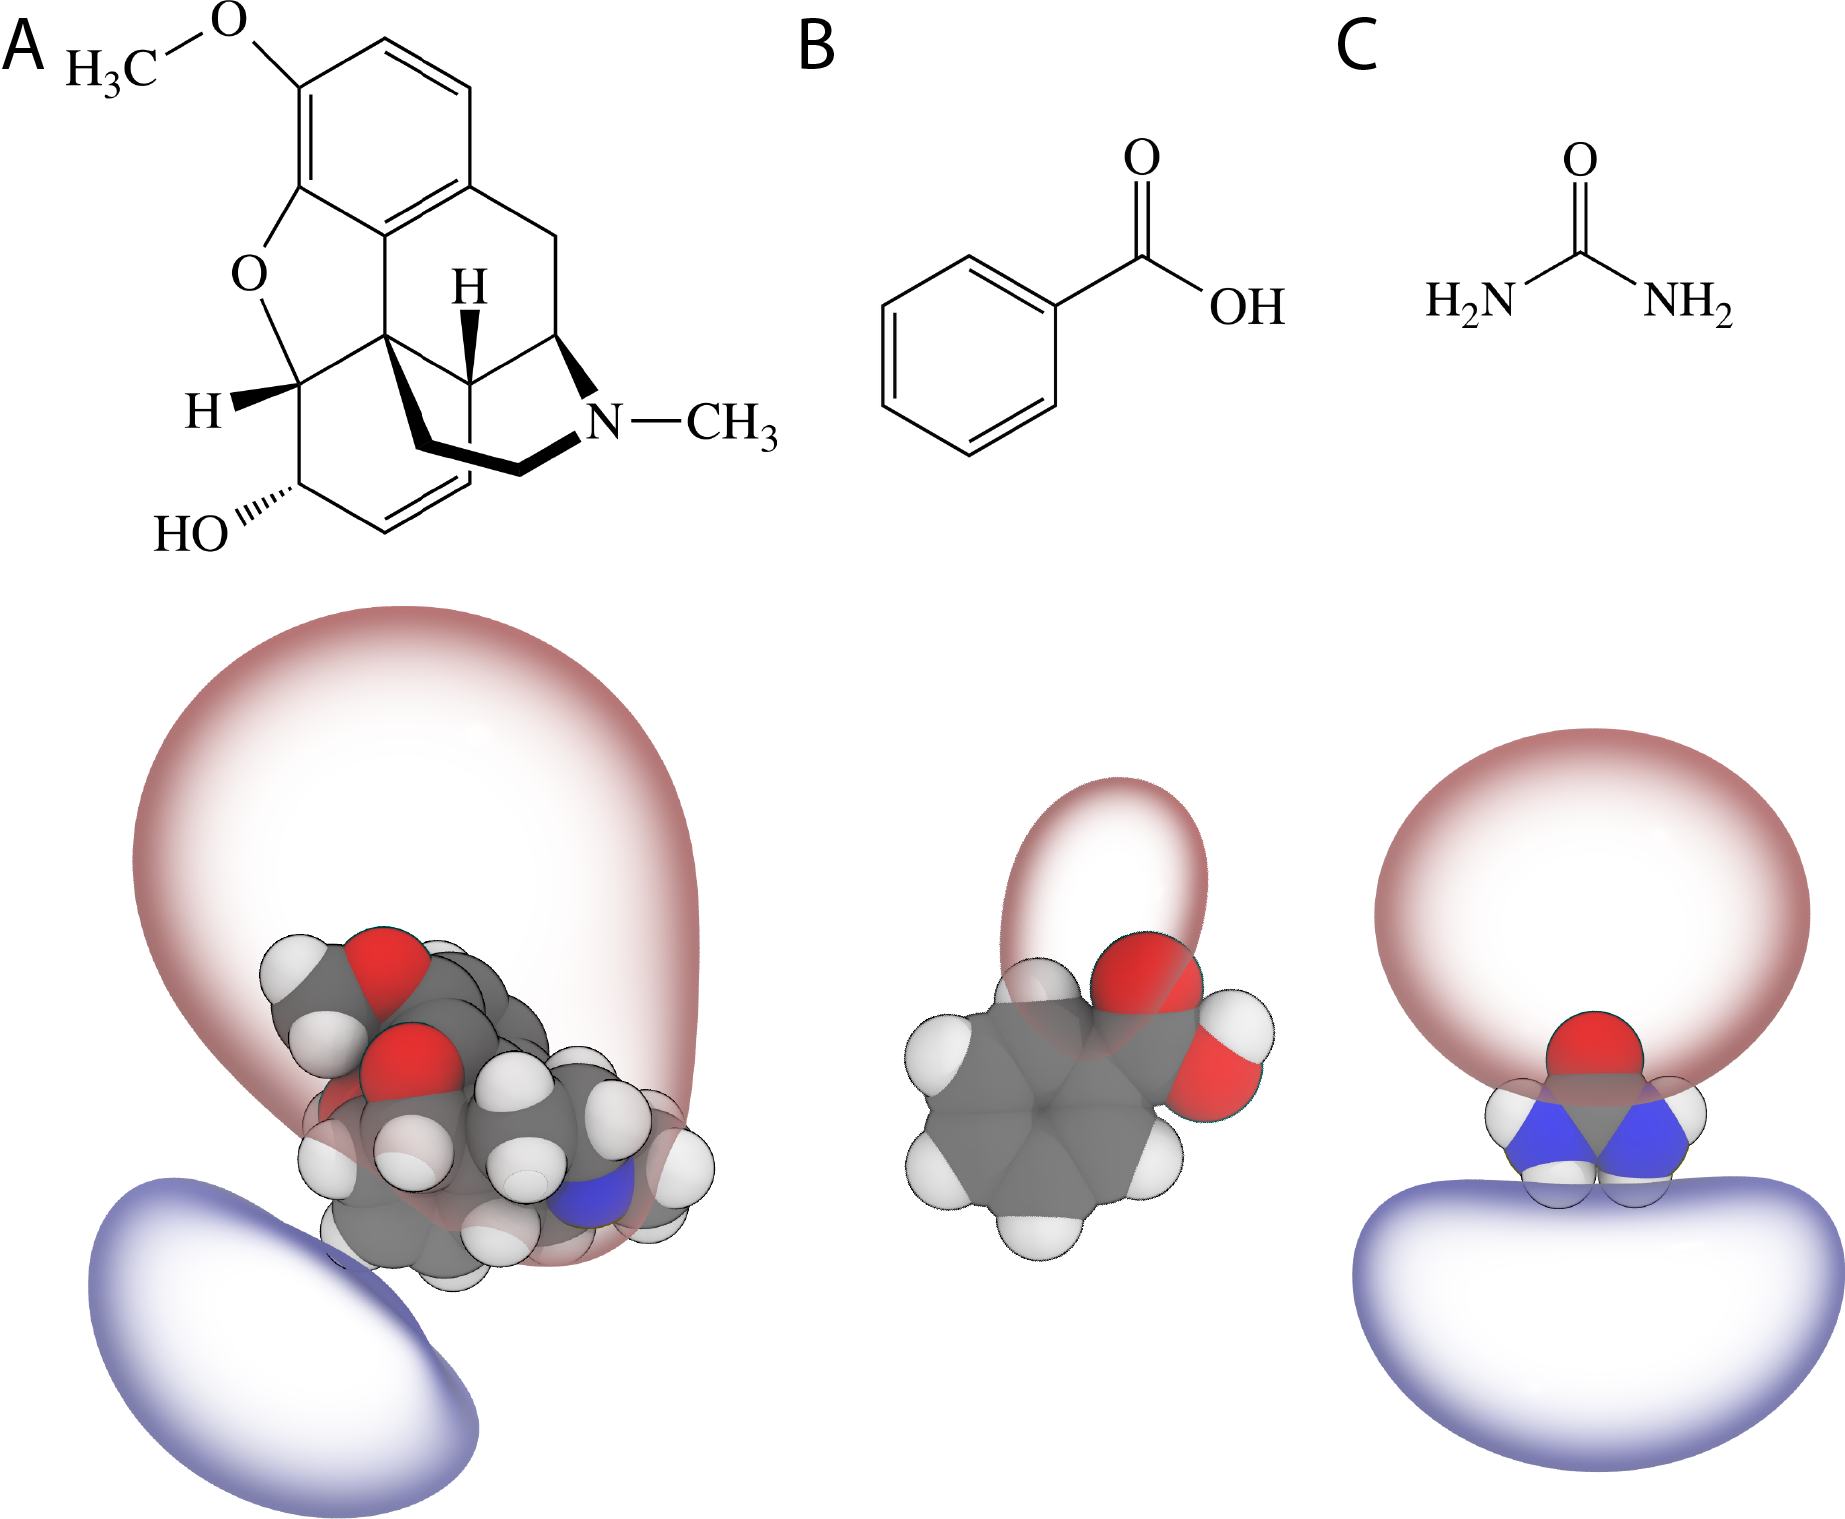
\includegraphics[width=0.6\textwidth]{Figures/permeants1}
\caption[Structures of permeants urea, codeine, and benzoic acid along with electrostatic potential isosurfaces]{Three permeants tested shown as 2D schematics (top) and 3D structures rendered with the $\pm 5$ kT/e electrostatic potential isosurfaces
using the assigned CGenFF charges (bottom).  (A) codeine.  (B) Benzoic acid (neutral).  (C) Urea.}
\label{fig:permeants}
\end{center}
\end{figure}

\subsection{Computed vs. experimental \perm}
\par The computed log\perm of the three permeants are listed in Table 1, along with the corresponding experimental references obtained from egg phosphatidylcholine bilayers (urea~\cite{Gallucci1971}, codeine~\cite{Orbach1980} and  benzoic acid~\cite{Walter1984}). From Table~1, it is clear that the majority of computed \perm values exceed the corresponding experimental data by 1--2 orders of magnitude. For comparison, we define $\Delta$log\perm = log\permcom - log\permexp, where log\permcom~and log\permexp~are the computed and experimental log\perm, respectively. Negative $\Delta$log\perm values are only observed for urea, the most hydrophilic of the three permeants.  Results obtained with different methods also show the largest discrepancy for urea: the US and REUS  methods underestimate log\perm by 0.87 and 0.51, whereas ABF and MW-ABF overestimate it by 0.71 and 1.14, respectively. For benzoic acid and codeine, all the methods overestimate log\perm by 0.71 to 1.67.


% \newcommand{\hl}[1]{\textbf{#1}}
% \providecommand{\e}[1]{\ensuremath{\times 10^{#1}}}

\begin{table}[h]
\centering
\caption[Estimated permeability values of permeants for each enhanced sampling strategy]{log\perm of the three permeants examined in this study. The unit of \perm is cm/s. Experimental values are obtained from \citenum{Orbach1980}, \citenum{Gallucci1971} and \citenum{Walter1984}.
For each computed log\perm, the length of the simulation used in the computation is shown in parenthesis.}
\begin{tabular}{@{}lccc@{}}
\toprule
& Urea & Benzoic Acid & Codeine     \\ \midrule
\textbf{Experiment} & -5.4          & -0.26                                             & -0.85      \\
\textbf{US}                & -6.27 (2.8\,$\mu$s)   & 0.45 (1.4\,$\mu$s)             & 0.03 (1.4\,$\mu$s)   \\
\textbf{REUS}              &  -5.91 (4.3\,$\mu$s)   & 1.17 (1.4\,$\mu$s)   & 0.64 (1.4\,$\mu$s)   \\
\textbf{ABF}               & -4.69 (0.9\,$\mu$s) & 1.16 (0.9\,$\mu$s)      &  0.82 (2.7\,$\mu$s)   \\
\textbf{MW-ABF}    &  -4.26 (1.4\,$\mu$s)   & 0.81 (0.7\,$\mu$s)       & 0.18 (1.1\,$\mu$s) \\ \bottomrule
\end{tabular}
\label{table:permresults}
\end{table}

Fig.~\ref{fig:deltaP} also reveals that with the possible exception of urea, increasing simulation time does not significantly improve agreement with experiment.  Even for urea, the computed \perm tends to plateau once the total simulation time exceeds 1\,$\mu$s.  It is unlikely that \perm has converged, however, but requires much longer time scales (milliseconds) to sample very slow membrane reorganization processes~\cite{Neale2011}.



\begin{figure}
\centering
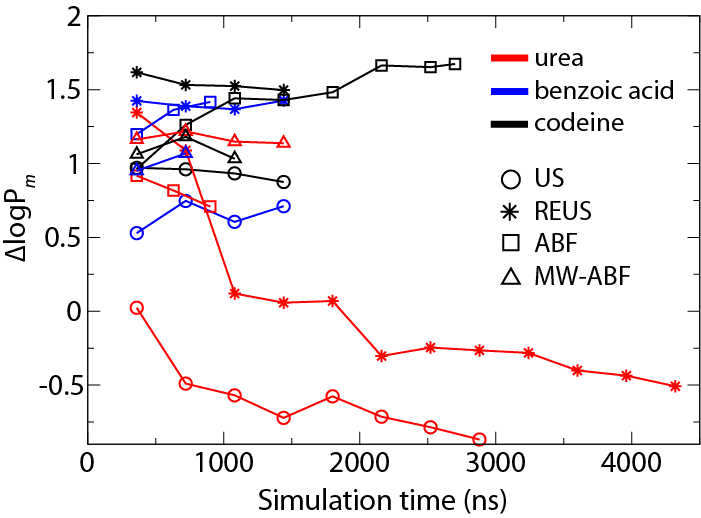
\includegraphics[width=0.65\textwidth]{Figures/dlogP-recolor.png}
\caption[Comparison of estimated permeability from four enhanced sampling methods]{$\Delta$log\perm of urea (red), benzoic acid (blue) and codeine (black) as a function of simulation time. Results obtained with different methods are indicated using the following symbols: US (circle), REUS (star), ABF (square), MW-ABF (triangle). }
\label{fig:deltaP}
\end{figure}


\subsection{Potentials of Mean Force}
\par In the solubility-diffusion model, the PMF is a critical component of the permeability (see Eq.~\ref{eq:solubility-diffusion}). Given its exponential weighting, the PMF may even be considered the greatest contributor to the permeability, making its accurate calculation of paramount importance.  To determine the best approach for calculating the PMF, we have compared four methods mentioned earlier and investigated the appropriate balance between equilibration time and sampling time.

\begin{figure}[htbp]
\begin{center}
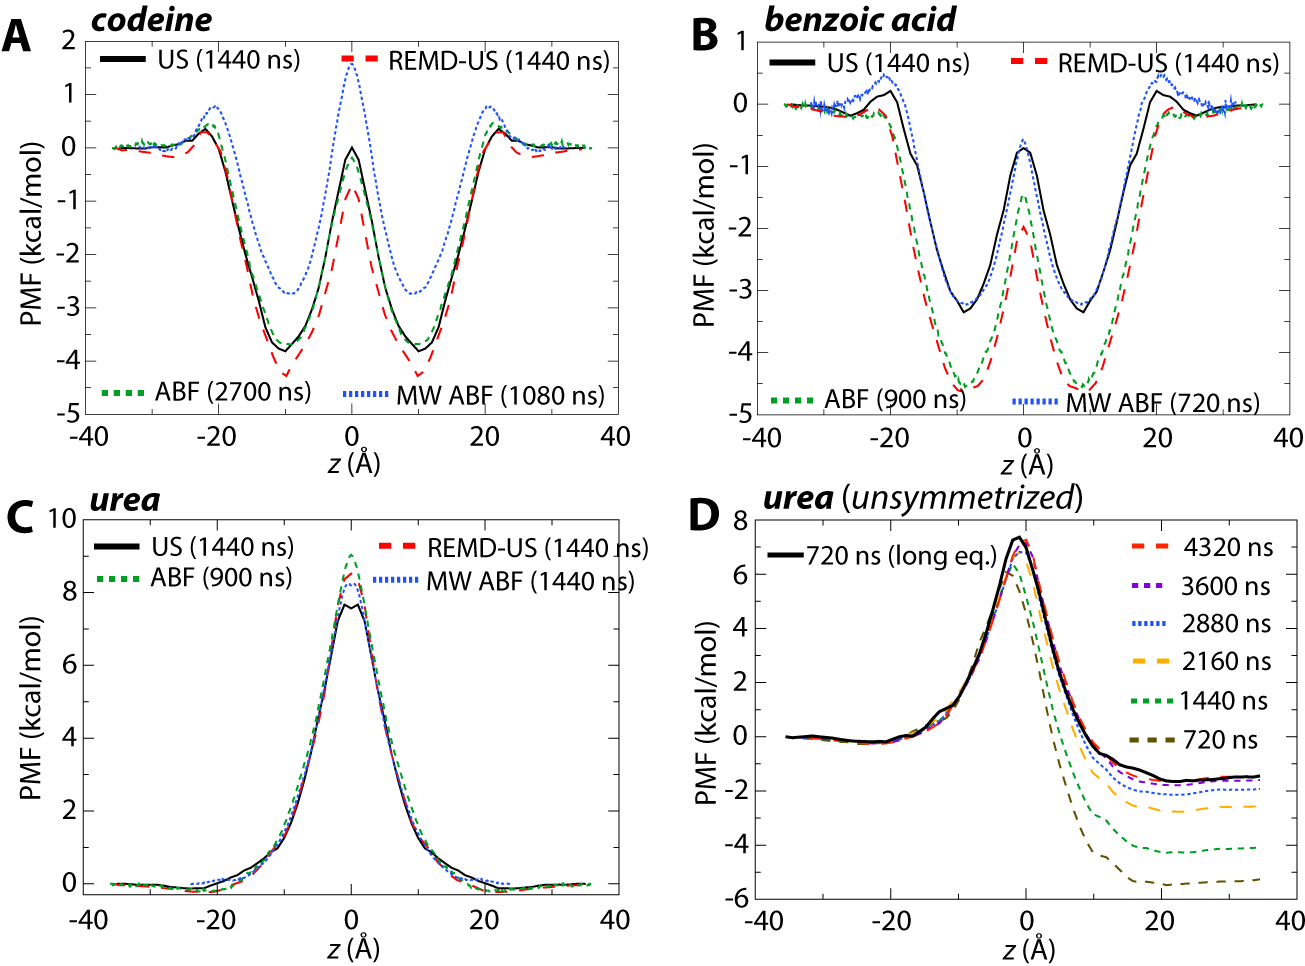
\includegraphics[width=0.8\textwidth]{Figures/PMFs-all}
\caption[Potentials of Mean Force for the permeants codeine, benzoic acid, and urea]{Potentials of Mean Force (PMFs) for the permeants (A) codeine, (B) benzoic acid, and (C) urea.  In each case, four PMFs from each of the methods are given: US (black, solid), REUS (red, large dashes), ABF (green, medium dashes) and MW-ABF (blue, small dashes).  All PMFs have been symmetrized about the membrane center.  (D) Convergence of the unsymmetrized PMF for urea.  PMFs determined using REUS for a total simulation time of 720\,ns -- 4.3\,$\mu$s are shown as various colored, dashed lines.  The PMF determined after 500\,ns of total equilibration and 720\,ns of sampling is also shown (solid black line) and is comparable to that from 4.3\,$\mu$s of sampling with less equilibration. See Fig.~S1 for the unsymmetrized PMFs for codeine and benzoic acid.}
\label{fig:PMFs}
\end{center}
\end{figure}

\par The PMFs were determined by bringing the permeant across the entire membrane and then symmetrizing the resulting profile, {\it i.e.}, the profiles were adjusted to be identical on either side of the membrane center and to both start and end at 0.  The resulting {\it symmetrized} PMFs for all three permeants are shown in Fig.~\ref{fig:PMFs}A-C.  Each plot shows varying levels of disagreement between the methods, although no method is consistently different.  For example, while for codeine, ABF and US are in agreement and MW-ABF is the most discrepant, for benzoic acid, MW-ABF and US are in agreement but different from REUS and ABF.  Thus, it is not apparent from these three permeants that any one method for determining the PMF converges more rapidly than the others.

\par The original profiles, prior to symmetrization, reveal a disturbing degree of asymmetry, and therefore accumulated error.  The evolving {\it unsymmetrized} profiles for urea are shown in Fig.~\ref{fig:PMFs}D and for codeine and benzoic acid in Fig.~S1.  After 720\,ns (10\,ns/window), the asymmetry between the two end points is $\sim$5\,kcal/mol.  This asymmetry decreases at a rate of only 1\,kcal/mol per 720\,ns, and still persists at $\sim$1.5\,kcal/mol after over 4\,$\mu$s of sampling. Trajectory snapshots from US of codeine bowing the interfacial phosphates as well as urea coordinating waters at the membrane core are shown in Fig.~S2 and S3, respectively, highlighting potentially slow converging orthogonal degrees of freedom.

\par One reason for the growing error in the PMF as the permeant goes through the membrane is the residual disturbance to the membrane structure from the steered MD used to generate the starting states. The time blocked probability distributions of headgroup phosphates and water in the vicinity of urea (shown in Fig.~S4) support the existence of non-equilibrium artifacts. One way to ameliorate this disturbance is longer equilibration of the starting states.  As a test of this idea, selected starting states for urea were equilibrated for a particular amount of time, dependent on their distance from the membrane center, namely 100\,ns at the center; 50\,ns at
$\pm$5\,\AA, $\pm$10\,\AA, and $\pm$15\,\AA; 25\,ns at $\pm$20\,\AA; 15\,ns at $\pm$25\,\AA; and 10\,ns at $\pm$30\,\AA,
giving a total of 500\,ns of equilibration.  Intermediate windows at each \aa ngstrom were then generated from these equilibrated states.  The unsymmetrized PMF resulting from 720\,ns of sampling with REUS is shown as the solid black line in Fig.~\ref{fig:PMFs}D.  It is immediately apparent that this newly generated PMF and its asymmetry after only 720\,ns are comparable to those after 4.3\,$\mu$s of sampling without sufficient equilibration.
Thus,
starting states should be sufficiently equilibrated in order to avoid artifacts resulting from their initial setup, in agreement with earlier recommendations by Palonc{\'{y}}ov{\'{a}} et al.~\cite{Paloncyova2012}.


\par In the preceding calculations, we determined the PMF for the entire permeation process, i.e., from $z=36$\,\AA~to $-36$\,\AA, after which the resulting PMF was symmetrized about the membrane center.  However, noting the expectation of a symmetric PMF, for many published cases the PMF is only determined from $z=36$ to 0\,\AA~\cite{Marrink1996,Bemporad2004,Holland2012}.  Given a finite amount of time for sampling, one may ask which is better --- to sample the full range of permeation for time $t$ or to sample half of the range for time $2t$ and then mirror it across the membrane center?  These two possibilities are compared in Fig.~S5.  When considering the {\it unsymmetrized} PMF from 10\,ns/window of the full range (10\,ns $\times$ 72 windows), the maximum value of 10.0\,kcal/mol is a full 1.8\,kcal/mol greater than the (presumably) converged result from 60\,ns/window (8.3\,kcal/mol).  For 20\,ns/window over half of the range (20\,ns $\times$ 36 windows), the maximum in the PMF is 9.4\,kcal/mol, apparently a better result than simulating over the full range.  However, once the result over the full range is symmetrized, the peak shifts to 8.0\,kcal/mol, significantly closer to the final result than the half-range peak.  Thus, the combination of simulating over the entire range along with the requirement of symmetrization appears to produce a more accurate result than simulating over half of the range for twice as long.


\section{Diffusivities}
\par The second key component of the solubility-diffusion model is the position-dependent diffusivity, $D$($z$). However, some commonly used methods for estimating diffusivity from simulations are not applicable to the heterogeneous membrane environment. One of the most common means of calculating the diffusion coefficient of a solute dissolved in a liquid is the Einstein--Smoluchowski equation. In the one-dimensional long-time limit, this equation relates the diffusivity, $D$($z$) to the mean square deviation of the position of the solute,
\begin{equation}
D(z) = \frac{\langle \left| z(t) - z(0) \right|^2 \rangle}{2t}.
\label{eq:einstein-smoluchowski}
\end{equation}
This relationship is only valid for solutes undergoing a random walk in a homogeneous liquid and offers a very poor approximation of the true diffusivity in a membrane, where most solutes encounter free-energy barriers with heights greater than $k_\mathrm{B} T$. For similar reasons, estimates based on a Green--Kubo relation of the velocity are expected to be equally poor~\cite{Mamonov2006}.

\par Marrink and Berendsen calculated the diffusivity profile for the permeation of water using the force autocorrelation function,~\cite{Marrink1994,Marrink1996}
\begin{equation}
D(z) = \frac{(k_\mathrm{B} T)^2}{\displaystyle \int_0^\infty \langle {\Delta}F_z(z,t)  {\Delta}F_z(z,0) \rangle \textrm{d}t}.
\label{eq:diff_marrink}
\end{equation}
This method requires that the solute be constrained to a point $z$ on the coordinate, which makes it relatively difficult to apply because the equations of motion of the MD integration must be modified to impose the constraint.~\cite{Wilson1985,Mamonov2006} As a result, it is far more common to perform simulations where the solute is simply restrained to remain near a given value of $z$ with a biasing potential. As the solubility-diffusion model requires the determination of $W$($z$) and $D$($z$) over the full bilayer, it would be preferable for the method used to provide both of these profiles from one set of simulations.

\par In the following sections, we present two strategies for calculating $D$($z$) for the permeation of a solute across a lipid bilayer using biased MD simulations. The first is based on the generalized Langevin equation for a harmonic oscillator. The second employs Bayesian inferences on the likelihood of the observed dynamics of the solute.

\subsection{The Generalized Langevin method}
\par The generalized Langevin equation provides straightforward methods to calculate
position-dependent diffusion coefficients from restrained MD simulations. In these methods, the solute is restrained by a harmonic potential so that it oscillates at a point along the coordinate. The solute can now be described as a harmonic oscillator undergoing Langevin dynamics, where the remainder of the system
serves as the frictional bath for the solute. Implicitly, describing the system as a harmonic oscillator requires the restraining potential to be dominant over the underlying free energy surface, i.e., the latter is effectively a perturbation on the former.
Otherwise,
the assumption that the bilayer serves only as a frictional bath to the oscillating solute may not be valid.  Values of the spring constant sufficiently large to justify this assumption also tend to be too large for umbrella sampling simulations, meaning that it may not be possible to use the same simulation to calculate $W$($z$) and $D$($z$).

\par Once a time series of the $z$ position of the solute is collected, the diffusion coefficient for that point can be calculated from the position or velocity autocorrelation functions (ACF and VACF, respectively).  These methods were originated by Berne and coworkers for the calculation of reaction rates~\cite{Berne1988}, and elaborated by Woolf and Roux to calculate position dependent diffusion coefficients.~\cite{Woolf1994} In their approach, the diffusion coefficient is calculated from the VACF. This approach requires the numerical Laplace transform of the VACF for several values of the transform parameter $s$ and extrapolation to the limit of $s=0$. Hummer proposed a simpler method to calculate diffusion coefficients from harmonically restrained simulations~\cite{Hummer2005} in which the diffusion coefficient is calculated directly  from the integral of the ACF, $C_{zz}$, of $z$ and the variance of $z$,

\begin{equation}
D(z= \langle z \rangle ) = \frac{\textrm{var}(z)^2}{\displaystyle \int_0^\infty C_{zz}(t) \, \textrm{d}t}.
\label{eq:diff_hummer}
\end{equation}

\par This method is attractive because it is simple to impose a harmonic restraint on a solute and save a time series of the $z$-position of this trajectory in most MD codes. It also avoids the need for multiple numerical Laplace transforms of the VACF. The ACF can be calculated directly from this time series,~\cite{Allen1989}
\begin{equation}
C_{zz}(t) =  \langle \delta z(0) \delta z(t) \rangle = \frac{1}{n_\mathrm{samples}}\sum\limits_{i=0}^{n_\mathrm{samples}} \delta z(i) \delta z(t+i)
\label{eq:correlation_sum}
\end{equation}
where $\delta z(t) = z(t)-\langle z \rangle$. Our code for calculating the ACF from a NAMD~\cite{Phillips2005}
time series is provided in the SI.
Although this method is a straightforward way to calculate membrane diffusion coefficient profiles, there are several practical issues associated with its use. We illustrate these issues by presenting the ACFs calculated from a simulation of urea restrained at three positions in the model bilayer system: $z=0$ \AA, $z=10$ \AA, and $z=36$ \AA\ (see Fig.~\ref{fig:acf}).

\begin{figure}
\begin{center}
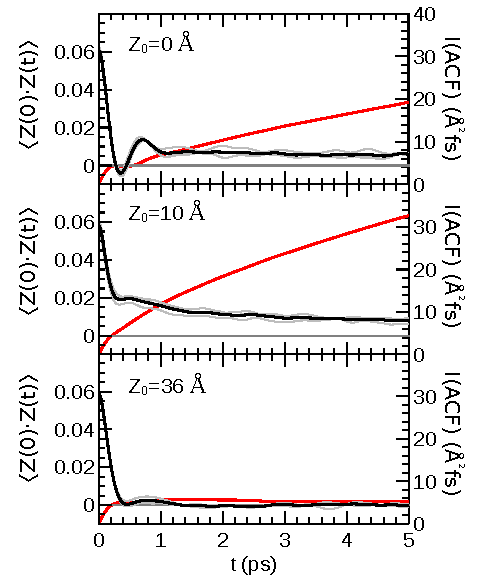
\includegraphics[width=0.65\textwidth]{Figures/acf-stacked}
\caption[Time autocorrelation function of urea in model DMPC bilayer]{Time autocorrelation function of urea in the model DMPC bilayer
restrained at various values of $z_0$ using a harmonic potential
($U_\mathrm{rest}=\frac{1}{2}k(z-z_0)^2$, $k=10$ kcal/(mol \AA$^2$)).
The black lines are the cumulative ACF calculated from three 1-ns simulations.
The ACF from each 1-ns trajectory alone is presented in grey. The red lines
(secondary axis) show the integral of the ACF over the interval $[0,t]$.}
\label{fig:acf}
\end{center}
\end{figure}

\par Correlation functions typically require extensive sampling to achieve convergence, particularly for long correlation times. Heterogeneity of the bilayer environment can cause the ACF calculated from different simulations at the same $z$-reference value to be significantly discrepant, a particularly serious for hydrogen-bonding solutes that remain partially coordinated by water molecules inside the membrane such as urea (see Fig. S3). This issue can be addressed in part by performing several simulations, with a long equilibration period for each. The correlation functions can then be calculated from long time series, e.g., > 1 ns, collected from each of these simulations.

\par The general features of the ACFs can be interpreted based on the analytical solution to the autocorrelation function of a harmonic oscillator undergoing Langevin dynamics,~\cite{Tuckerman2010}
\begin{equation}
C_{zz}(t) = \textrm{var}(z) e^{-\gamma(\bar \omega)t/2\mu}[ \textrm{cos}(\Omega t) + \frac{\gamma(\bar \omega)}{2 \mu \Omega } \textrm{sin}(\Omega t)]
\label{eq:analytical-acf}
\end{equation}
where $\gamma$ is the friction coefficient, $\bar \omega$ is the renormalized frequency of the oscillator, and $\mu$ is its reduced mass. $\gamma$ determines the rate of decay of the ACF. The expected behavior of the ACF based on Eq.~\ref{eq:analytical-acf} is that for damped periodic oscillations; however, if the friction coefficient, $\gamma$, is high, the ACF may decay to zero before there are any significant oscillations. This decay is apparent in the ACF when the solute is restrained at  $z=36$ \AA\ (bulk water; see Fig.~\ref{fig:acf}), which decays to zero within 0.5 ps, but then has a short second peak extending to 1.2 ps. The calculation of the diffusion coefficient formally requires the integration of the ACF in Eq.~\ref{eq:diff_hummer} over the interval $[0, \infty]$, but the ACF will  decay to zero within $\sim$ 2 ps in most fluid environments. Even if extensive sampling has been performed, there can be significant noise in the ACF at long times. Hummer noted that this noise causes the calculated diffusion coefficients to be sensitive to the interval of integration.~\cite{Hummer2005} The g\_wham code~\cite{Hub2010}, one of the tools provided with Gromacs, limits the contribution of noise by cutting off the integration when the ACF drops below a threshold value of $0.05\ \times\ \textrm{var}(z)$.  This cutoff is not appropriate in all instances because the ACF can go through multiple oscillations before converging to zero. Nevertheless, it can provide reasonably accurate results if the autocorrelation function decays rapidly (i.e., in a high friction regime).

\par Compared to bulk water, the autocorrelation functions in the lipid tail region are much slower to converge.  The ACFs from simulations with $z_0=10$ \AA\ and $z_0=0$ \AA\ only decay to 8 and 13\% of their initial values in 5 ps, respectively. A consequence of the
failure to converge to zero is that the integrated ACF increases almost linearly,
causing the calculated diffusion coefficients to be sensitive
to the interval over which the ACF is integrated.  Typically, this sensitivity will cause
the integrated ACF to be larger than it should be, so that the calculated diffusion coefficient is erroneously underestimated.

The slow convergence of the ACF is consistent with the work of Neale et al.,~\cite{Neale2011}
which showed that the convergence of US simulations of solute permeation
into bilayers can require $\mu$s-ms-length simulations. Long correlation times are
due to slow diffusion of the lipid tails, variations in the hydration of the solute, and
inhomogeneities in the bilayer interface that form over very long time scales.~\cite{Neale2013}
While US simulations of the bilayer PMF can achieve convergence by running for a very long time, the
lack of ergodicity in sampling is inconsistent with the underlying model of harmonic
oscillator in frictional bath that is used to derive Eq.~\ref{eq:diff_hummer}.

The issues noted above for calculating diffusivity in the membrane are typically not
significant for small solutes like water,~\cite{Riahi2014,Issack2015}
but they are severe for larger, more complex ones, such as urea, which are more prone to
have long-time correlations. Under such circumstances, the Generalized Langevin method is not appropriate for
calculating $D$($z$).  To determine if convergence issues are significant for a given
system, the ACF should be calculated and plotted for several $z$-positions in the bilayer. If the ACF
has not decayed to values near zero at long time scales (e.g., 5 ps), the Generalized Langevin
method is probably not appropriate for calculating the position-dependent diffusivity for that solute.

In the Generalized Langevin approach, a prerequisite noted above is that the force constant
of the harmonic restraint should be sufficiently large to render the underlying free-energy
surface a small perturbation on the harmonic potential.  The force constant used for the US
simulations, 1.5\,kcal/mol/\AA$^2$, may be
too small for application of this approach.  To test its applicability, we ran additional
2-ns simulations for each window for urea using a much larger restraining force constant
of 10\,kcal/mol/\AA$^2$.  However, as shown in Fig.~S6, the differences
between the $D$($z$) profiles for the two cases are practically negligible at nearly all
points.  At a few data points in the membrane interior, urea under a higher restraint
gives a diffusivity as much as twice that of urea under a lower one.  Yet, because
the permeability depends linearly on $D$($z$) (see Eq.~\ref{eq:solubility-diffusion}), but
exponentially on $W$($z$), even a factor of two in the diffusivity across the entire permeation
pathway contributes only $\sim$0.3 to log\perm.  Thus, for permeability calculations, it is
acceptable to use the same simulations for calculation of both $W$($z$) and $D$($z$).

\subsection{The Bayesian inference method}



A fundamentally different approach for the determination of position-dependent
diffusivities employs Bayesian inferences to reconcile thermodynamics and kinetics~\cite{Hummer2005,Turkcan2012,Comer2013}.  This approach is especially suited for calculations within lipid membranes
because no assumptions are made regarding the form of the free-energy landscape on which diffusion occurs.
Furthermore, such an approach
is compatible with a wide variety of biasing schemes used in MD,
and thus, allows the practitioner more flexibility in simulation design.
This approach may be viewed as the
inverse solution of the Smoluchowski equation, which yields consistent estimates
of $W$($z$) and $D$($z$), given the
trajectory obtained from biased simulations.
These biases may also be time-dependent, as is the case for
the metadynamics and ABF algorithms.
Since the latter free-energy calculation algorithms are
designed for the accurate description of $W$($z$), one may use it as a
consistency check of the solution provided by the Bayesian inference method.
Alternatively, $W$($z$) as determined by a free-energy algorithm can
serve as a prior in the Bayesian scheme, increasing the reliability of
$D$($z$) in situations where statistics are poor.
In a nutshell, the Bayesian scheme uses as parameters the values of
the transition coordinate, $z$, along the trajectory, together with the force, $F(z,t)$,
which is the sum of the time-dependent bias and the intrinsic system force, equal
to $-\nabla W(z)$. Under the stringent assumption of a diffusive regime, the
motion is propagated using a discretized Brownian integrator,
\begin{equation}
\Delta z = z_2(t) - z_1(t) = \beta D(z_1) F(z_1, t_1) \Delta t + \nabla D(z_1) \Delta t + \sqrt{2 D(z_1) \Delta t} \ g(t)
\label{Brownian}
\end{equation}
where $\beta = (k_B T)^{-1}$, $\Delta t = t_2 - t_1$ and $g(t)$
is a Gaussian white noise of zero mean and variance equal to unity. Propagation along the
transition coordinate can be recast as the sum of a drift and a noise
term, i.e., $\Delta z = \mu + \sigma g(t)$, where
$\mu$ and $\sigma^2$, the variance, are defined by,
\begin{equation}
\left\{
\begin{array}{lcl}
\mu      & = & \beta D(z_1) F(z_1, t_1) \Delta t + \nabla D(z_1) \Delta t
\\
\sigma^2 & = & 2 D(z_1) \Delta t
\end{array}
\right.
\end{equation}
Propagation of motion obeys a Gaussian-distributed probability of observing the
transition from $z_1$ at time $t_1$ to $z_2$ at time $t_2$,
\begin{equation}
\label{eq:Gaussian}
P[(z_2, t_2 | z_1, t_1) | F(z,t), D(z)] =
\frac{1}{\sigma \sqrt{ 2 \pi}}
\exp \left(-\frac{(\Delta z - \mu)^2}{2 \sigma^2} \right)
\end{equation}
which assumes the system is in the overdamped Langevin dynamics regime and satisfies the
fluctuation-dissipation theorem.
It is worth noting that in contrast with related
schemes, the present formalism, embodied in Eq.~\ref{Brownian}, features
a gradient term, $\nabla D(z_1) \Delta t$, which has been shown to improve
the accuracy of the predicted intrinsic system force, or gradient of the PMF.
See the SI for more details on applying the scheme
to MD simulations.

As shown in Fig.~\ref{fig:acf}, the motion of permeants within the membrane is complex and correlations in such motion are much longer in the membrane environment than in solutions (at least several picoseconds).
These long correlation times complicate calculating the diffusivity by most
available methods, including the Bayesian inference method described herein.
A crucial component of this scheme is the time step, $\Delta t$.
The correlations shown in Fig.~\ref{fig:acf} violate the assumptions of
overdamped Brownian motion leading to Eq.~\ref{Brownian}; thus,
we found that $\Delta t$ values of a few picoseconds yield substantial overestimates of the diffusivity.
$\Delta t$ should be chosen to be much larger than any correlation
time of the motion; however, there is also an upper bound on $\Delta t$ because
the discretization implicit in Eq.~\ref{Brownian} requires
only small changes in $F(z_1, t_1)$ and $D$($z$) over the duration of $\Delta t$.
Errors due to the violation of this requirement are apparent when
$W$($z$) as predicted by the Bayesian scheme diverges substantially
from that obtained by the free-energy calculation technique
(here, ABF).
For the permeants examined in the present work,
we found $\Delta t=32$~ps still gives consistent $W$($z$)
functions while minimizing errors due to correlation.

\subsection{Comparison of the two approaches}
As is clear from Eq.~\ref{eq:solubility-diffusion}, log\perm is much more sensitive to $W(z)$ than to $D$($z$).
However, as shown in Fig.~\ref{fig:Dz}, there are some notable differences
in the results of the Generalized Langevin and Bayesian inference approaches, which
have an appreciable effect on the predicted permeability.
For the four methods used to determine the PMF, the Generalized Langevin approach
for calculating $D$($z$) was used for US and REUS, while the Bayesian inference method
was used for ABF and MW-ABF.
Under the conditions described above, i.e. the restraint strength used in the US and REUS
simulations and the $\Delta t$ chosen for the Bayesian scheme,
we obtain smaller diffusivity values using
the Generalized Langevin approach than using the Bayesian approach.
These differences are most notable near $z=0$, where the value of $D$($z$)
most influences the permeability for urea due to the maximum of $W$($z$).
For example, the much larger diffusivity of urea
near the center of the membrane as determined by the Bayesian scheme
compared to the Generalized Langevin scheme (see Fig.~\ref{fig:Dz})
results in the ABF and MW-ABF methods having larger log\perm values by more than
an order of magnitude, despite the fact that the
height of the free energy barrier calculated by ABF is significantly
larger than that for the other methods (see Fig.~\ref{fig:PMFs}).
The generally larger $D(z)$ values given by
the Bayesian scheme are likely due to the fact that
the scheme used in the present work is limited to relatively small values of $\Delta t$, a consequence of the Gaussian approximation for the probability profile (Eq.~\ref{eq:Gaussian}). We have found that the motion of the permeants is not strictly diffusive at the $\Delta t$ values used here and that the diffusivity appears to decrease continuously with $\Delta t$. We are currently working to improve the Bayesian scheme to overcome the limitations on $\Delta t$, which will be addressed in subsequent work.
Hence, although it plays a less dramatic role in Eq.~\ref{eq:solubility-diffusion} than $W$($z$),
$D$($z$) is also highly influential and the approach to calculating it must be
carefully considered.

\begin{figure}[htbp]
\begin{center}
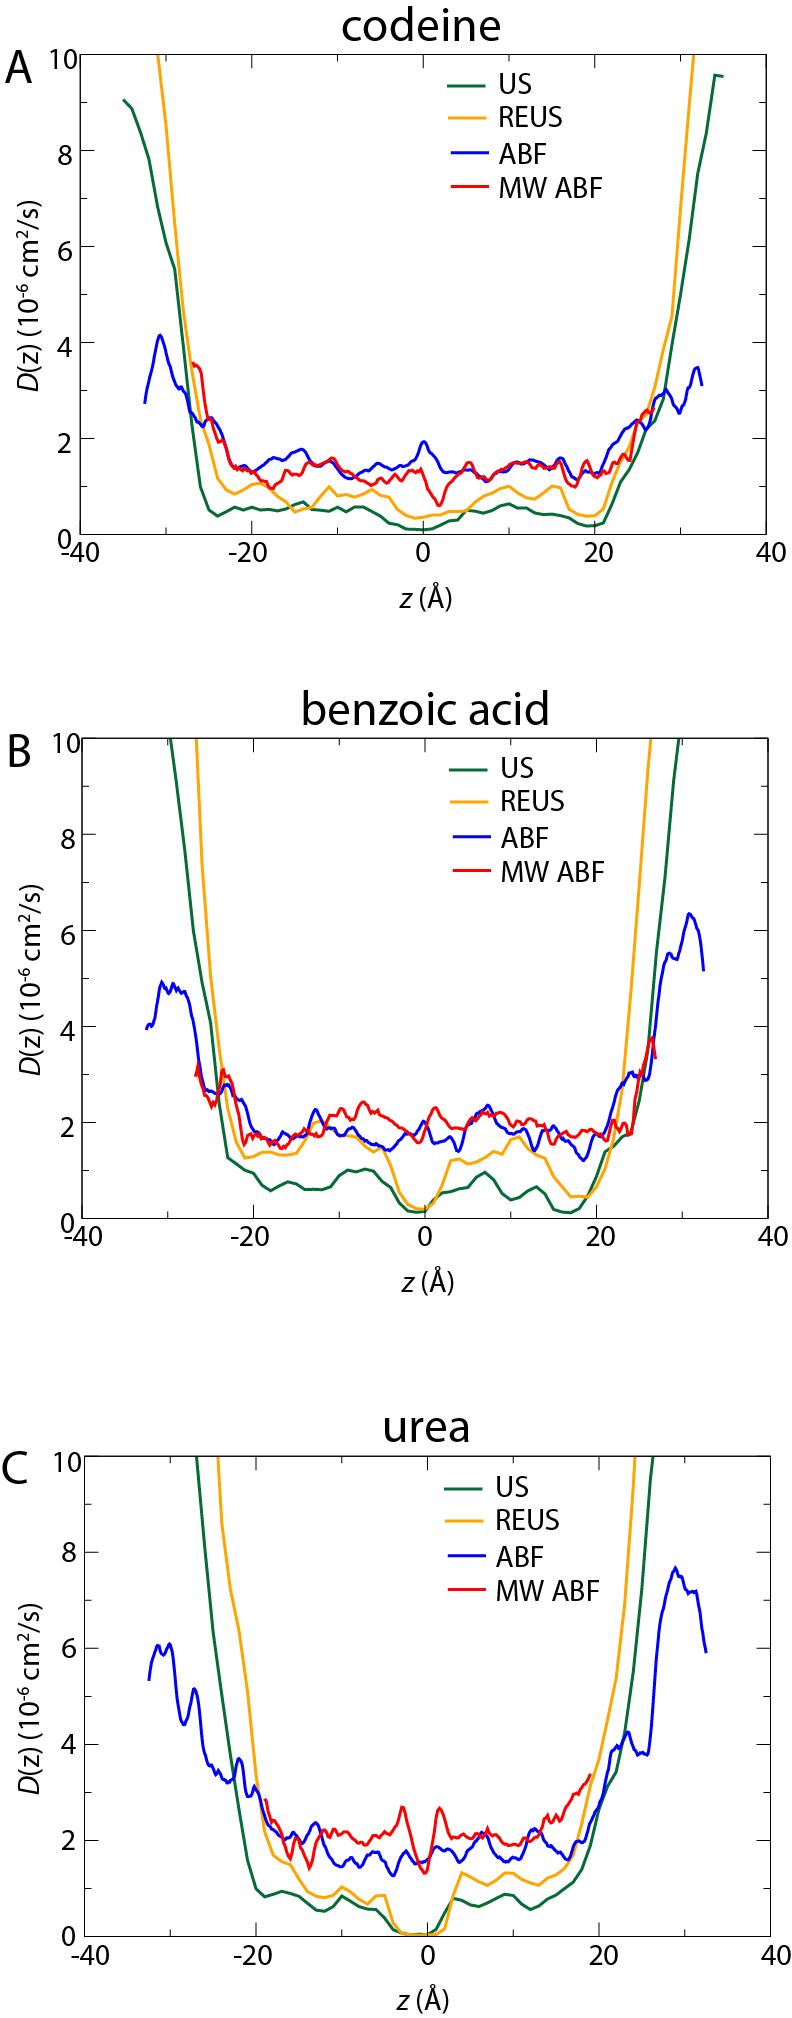
\includegraphics[width=0.4\textwidth]{Figures/Dz-all}
\caption[Diffusivity profiles for permeants urea, benzoic acid, and codeine]{Diffusivity profiles for each permeant, (A) codeine, (B) benzoic acid, and (C) urea.  In green and orange are the umbrella-based methods, US and REUS, for which the Generalized Langevin approach was used to determine $D$($z$).  In blue and red are the ABF-based methods, for which the Bayesian scheme was used.}
\label{fig:Dz}
\end{center}
\end{figure}

\section{Comparison of methods and tolerance to error}
\par Results presented up to this point do not favor any one method over another.  For example, while REMD-US is more accurate for urea, it is less so for the other two permeants (see Table~\ref{table:permresults}).  To examine if the rate of convergence depends on the method employed, we have plotted for each method and permeant log\perm as a function of simulation time in Fig.~\ref{fig:deltaP}.  For codeine and benzoic acid, the variance in log\perm for a given method is quite small, no more than 0.25 log units, even between 360\,ns and almost 3\,$\mu$s, suggesting that as much as 90\% of the simulation time invested was unnecessary.  On the other hand, there is a clear effect of time on log\perm for urea, with it changing by as much as two log units over time.   The downward trend for urea's log\perm is an effect of the shrinking peak in the PMF (Fig.~\ref{fig:PMFs}C).   A similar trend for codeine or benzoic acid is likely not observed because the peaks in their PMFs, i.e., those parts above 0 that contribute most significantly to log\perm, are almost non-existent.   Regardless, for codeine and benzoic acid, the disagreement with experiment is notable in part because the simulated values are consistently greater by 0.5 to 1.5 log units.


\par After examining the PMFs and diffusivities in great detail, it is useful to consider their individual contributions to the permeability and, thus, how accurate each of them ought to be to give log\perm at a chosen level of accuracy.  To explore how these two parameters contribute to the permeability, a program to generate arbitrary PMFs and diffusivities was written.  This program creates smooth profiles based on input values of the PMF and diffusivity at the interfacial region and at the center of the membrane (see Methods for more details).  We first used the program to test molecules with a single barrier (or valley) at the membrane center, varying the barrier's height and width.  As seen in Fig.~\ref{fig:models}A, the contribution of the width is negligible, while the height of the barrier dominates log\perm.  For positive PMF values
at the center, there is roughly a correspondence of 2\,kcal/mol to one log unit for log\perm.  Changing the diffusivity by a factor of 10 (range of $10^{-6}$ to $10^{-5}$\,cm$^2$/s) has a similar effect of one log unit, as expected from the linear dependence of the permeability on $D$($z$) (see Fig.~\ref{fig:models}B).  Nearly identical behavior was observed when two barriers were placed at the interfacial region, with only the height and not the position of the barriers contributing (see Fig.~S7).

\begin{figure}[htbp]
\begin{center}
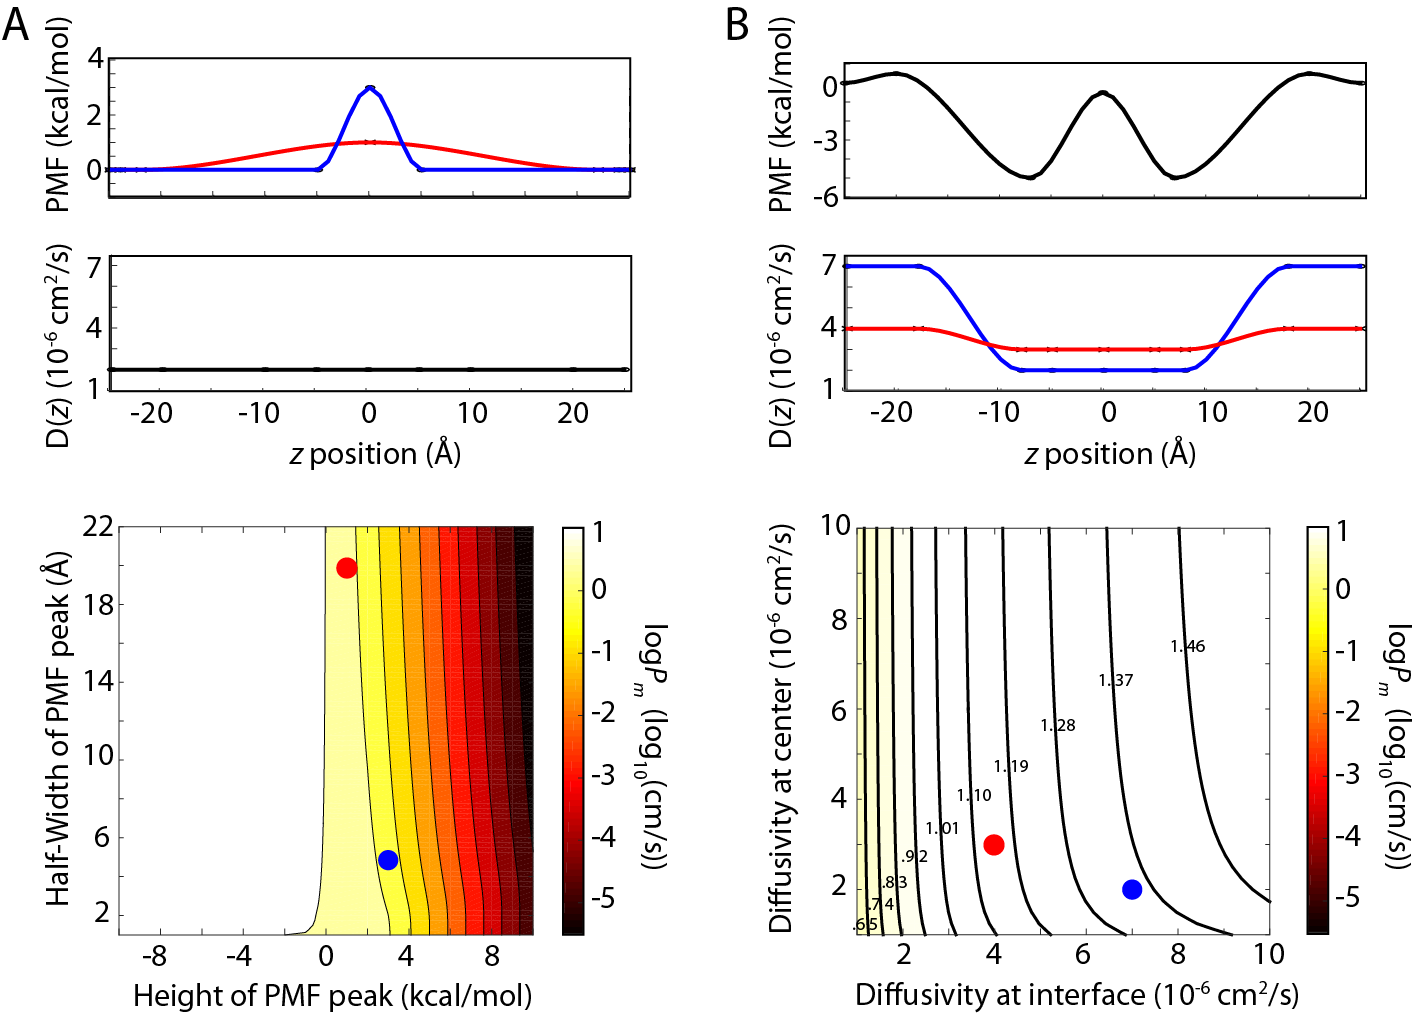
\includegraphics[width=0.9\textwidth]{Figures/models}
\caption[log\perm as a function of modeled inputs]{log\perm as a function of modeled input.  In both parts, the input PMF and $D$($z$) are shown on top and the dependence of log\perm on them on bottom.  In each contour plot, the red and blue circles correspond to the red and blue PMF or diffusivity above.  (A) log\perm as a function of PMF barrier height and width.  $D$($z$) is held constant.  (B) log\perm as a function of diffusivity profile.  The PMF is held constant.  $D$($z$) is varied at $z=\pm 20$\,\AA~(interface) and at $z=0$\,\AA~(center).  The range of log\perm values is 0.55 to 1.55, with contour values given in the figure.}
\label{fig:models}
\end{center}
\end{figure}

\par While permeants for which the PMF barrier is pronounced have their log\perm values dominated by the barrier height, others may exhibit more subtle dependencies.  To test this possibility, a PMF in which the barriers are less than 1\,kcal/mol at the interfacial regions of the membrane, akin to the PMFs for codeine or benzoic acid, was created and the diffusivity profile varied.  As shown in Fig.~\ref{fig:models}B, the diffusivity at the PMF barriers contributes to log\perm, but that at the core (a minimum in the PMF) does not.  As a final test of the minimal amount of information necessary to calculate log\perm, we generated PMFs and diffusivities to match those from simulation based solely on the PMF value at the peak(s) and $D$($z$) at that position.  Comparison of each generated profile to the computed ones is presented in Fig.~S8.  The obtained log\perm values are 0.31 (benzoic acid), 0.44 (codeine), and $-5.82$ (urea).  While urea is identical to the value estimated with REUS (see Table~\ref{table:permresults}), the other two permeants are slightly below their computed values (difference of 0.85 and 0.63, respectively), although they are closer to experimental values.  Regardless, our models demonstrate that log\perm can be obtained from surprisingly few data points to a high degree of accuracy.

\par In lieu of determining the full PMF, which can require microseconds of simulation, one can use alternative methods to sample the critical points, i.e., at the interface and/or at the center.  As a proof-of-concept, we ran alchemical free energy perturbation (FEP) to calculate the solvation free energy of urea in the membrane core and in water.  We found $\Delta G = 9.26$\,kcal/mol ($\sim$1--1.5\,kcal/mol higher than predicted by our PMFs in Fig.~\ref{fig:PMFs}) and $D(0) = 1.25\times 10^{-6}$\,cm$^2$/s.  When combined with a very simple interpolated PMF curve that goes smoothly to 0 at $z=\pm20$\,\AA, we find log\perm = $-5.26$.  This is within < 3\% of the experimental value, despite requiring significantly less simulation time: 200\,ns for FEP vs. at least 1\,$\mu$s for the full-PMF approach.  However, one loses insight into the details of the permeation process when using FEP over a PMF-based method.




\section{Conclusions}

We have computed the membrane permeability to three compounds using a variety of simulation-based methods, namely US and ABF, along with their multiple-copy variants, REUS and MW-ABF, respectively.  These three compounds, codeine, benzoic acid, and urea, span a range of chemical properties and, most importantly, permeabilities (see Table~\ref{table:permresults}).  All simulation methods were able to predict the permeability within one log unit typically, except in a few cases that were off by 1.5 (see Fig.~\ref{fig:deltaP}).  Interestingly, of the four methods tested, none stood out as unequivocally better than the others.  The root-mean-square error in log units for each method was 0.821 (US), 1.23 (REUS), 1.33 (ABF), and 1.08 (MW-ABF).

Because of their similar performances, no one simulation method is recommended over another.  However, regardless of the method chosen, certain procedures can improve convergence.   It was found that simulation over the entire range, i.e., from one side of the membrane to the other, followed by symmetrization of the resulting PMF converged much faster than simulating over just half the range, i.e., from one side to the membrane center (see Fig.~S5).  Additionally, the states used to seed the windows for production sampling should be well equilibrated.  Methods such as SMD used to produce these initial states induce significant non-equilibrium perturbations to the membrane that may take hundreds of nanoseconds or more to equilibrate.  Alternatives to SMD include building the membrane {\it de novo} around the permeant at varying depths~\cite{Dorairaj2007} or introducing the permeant in a perturbative fashion at different values of $z$.  Regardless of the method, equilibration should be carried out for as long as is feasible (50-100\,ns/window at least, depending on membrane depth), particularly when the permeant's stability relies upon the spontaneous formation of membrane defects and penetration of water.

Two methods for calculating the diffusivity were explored.  The first, more commonly used Generalized Langevin method, based on restraining the solute and measuring the correlation of the system forces acting on it, was combined with the PMFs in the US and REUS; the second, the Bayesian inference method, was combined with PMFs from ABF and MW-ABF.  Both methods present a number of subtleties that prevent a straightforward calculation of $D$($z$), e.g., a proper choice of the force constant in the Generalized Langevin method or the discretization time step in Bayesian inference.  Furthermore, they are both plagued by long correlation times that are not amenable to the usual MD time scales.  Despite these caveats, they produced diffusivity profiles in rough agreement, although those from the Bayesian inference method are consistently slightly higher in the membrane than those from the Generalized Langevin method (see Fig.~\ref{fig:Dz}).

Because the solubility-diffusion model relies on two position-dependent quantities, the PMF and the diffusivity, it is natural to assume they must be calculated to determine the permeability.  However, as demonstrated in the section ``Comparison of methods and tolerance to error'', only a few data points contribute significantly to it.  Therefore, permeability can be estimated from a handful of parameters, namely the values of $W$($z$) and $D$($z$) at the membrane/water interface and at the membrane center, with the remainder interpolated from an expected smooth topology.  Going even further, extrapolating from just a single value each of the PMF and the diffusivity at the membrane center for urea (see Fig.~\ref{fig:models}A) produced a log\perm almost identical to the experimental value.  Thus, we recommend that sampling be focused on critical regions where barriers are expected, e.g., the membrane core and/or interfacial region.

Taken together, the results show the robustness of a variety of MD-based methods in calculating membrane permeability for small molecules.  In particular, all methods appear to converge on sub-$\mu$s time scales, although the determined log\perm values are nearly all 0.5 to 1.5 log units above the experimental values.  This consistent overestimation is in agreement with a previous MD study from 2004~\cite{Bemporad2004}, despite using 10-100$\times$ longer simulations in the current study.  The membranes compared, DMPC in simulation with egg PC in experiment, are not identical, which may contribute to the discrepancy.  Another possible reason could be slow membrane reorganization that occurs on a time scale even an additional 2-3 orders of magnitude greater~\cite{Neale2011}.  The lack of polarizability is another tempting possibility, given the vastly different environments experienced by the permeating molecule~\cite{Riahi2014}.
Similarly, the most commonly used force fields (including CGenFF used in this study) are primarily parameterized to reproduce phenomena obtained in aqueous environments. Thus, it may be unrealistic to expect that solute phenomena within the non-polar membrane environment is as well represented. Therefore, further exploration of the force-field effects within lipid-like or non-polar environments are warranted.  In particular, inclusion of explicit polarizability may improve accuracy, although at a computational cost of 2-6$\times$~\cite{Chowdhary2013,Wang2013}. However, given the lack of convergence of the four methods to a single value for each permeant, all of which use the same force field, it cannot be known a priori to what degree, if any, changes to the force field will improve agreement with experiment.
Additionally, the assumptions of the solubility-diffusion model, such as the reliance on a single reaction coordinate and that permeation obeys classical diffusion, may need to be challenged to obtain improved quantitative agreement with experimental measures~\cite{Orsi2010,Parisio2013,Comer2014}.

Finally, we draw attention to the potential benefit of our results to QSPR models.
We have shown that only one or two points in the PMF and diffusivity contribute significantly to the permeability.  Thus, calculations for a single permeant focusing on these critical points could be done in hours on a sufficiently fast cluster.  Furthermore, the location of these points, typically at the membrane center or at the water/membrane interface, suggest reduced systems that could represent them reasonably well, e.g., octanol for the interfacial region.
Combined with improved force fields, fast calculations on such reduced systems could augment the molecular descriptors used to design QSPR models, similar to the ``membrane-interaction QSAR'' approach pioneered by Hopfinger et al.~\cite{Kulkarni1999,Tseng2012}.

\section{Methods}

\subsection{System preparation}

\par We constructed a model membrane bilayer consisting of pure dimyristoyl phosphatidylcholine (DMPC) using the CHARMM-GUI membrane builder~\cite{Wu2014a}. The membrane consists of 64 lipids per leaflet solvated by 30-\AA~water pads on either side. The number of lipids was selected to provide balance between the accuracy of the free energy calculations and the bilayer size~\cite{Hu2013}. All simulations were run using TIP3P water~\cite{Jorgensen1983} and CHARMM36 lipid parameters~\cite{Klauda2010}. Previously it has been identified that CHARMM36 is a good choice for small molecule permeability calculations~\cite{Paloncyova2014}.  Small-molecule parameters came from the CGenFF force field~\cite{Vanommeslaeghe2010}.  In the case of codeine, which is not part of the standard CGenFF distribution, compatible parameters were obtained from the Paramchem webserver~\cite{Vanommeslaeghe2012,Vanommeslaeghe2012b}.

\par The membrane-water system was minimized and equilibrated in multiple stages. During the first stage, the membrane was constrained and water was allowed to minimize for 5,000 steps. During the second stage, the membrane was allowed to minimize for 5,000 steps and the water was constrained. During the third stage, both the water and membrane were minimized for 10,000 steps in the absence of constraints. Following minimization, 10 ns of NPT equilibration was carried out using a Lowe-Andersen thermostat~\cite{Koopman2006,Lowe1999} and Langevin barostat~\cite{Feller1995} at a temperature of 298.15 and pressure of 1 atm. The Lowe-Andersen cutoff and coupling rate was set to 2.7 \AA~and 50 ps$^{-1}$, respectively. The barostat period and decay times were set to 100 and 50 fs respectively. A 2-fs time step was used. The SETTLE algorithm~\cite{Miyamoto1992} was used to constrain all covalent bonds to hydrogen atoms. The long-range cutoff was set to 12~\AA, and short-range non-bonded and bonded interactions were calculated every time step. Long-range electrostatics were calculated using the Particle Mesh Ewald method~\cite{Darden1993} every two time steps.  All minimization, equilibration, and production dynamics were carried out using the NAMD molecular dynamics engine~\cite{Phillips2005}.

Steered MD~\cite{Izrailev1997,Sotomayor2007} simulations were used to pull each permeant through the membrane at a speed of 0.7\,\AA/ns (100\,ns in total).  Coordinates of the system with the permeant at equally spaced locations over the permeation pathway were extracted from the trajectories and used as initial states for all subsequent simulations.

\subsection{Umbrella Sampling}

\par The reaction coordinate was defined as the $z$-component of the distance separating the center of mass of lipid phosphorous atoms and the heavy atoms of the permeant. For each of the permeants, a total of 71 windows spaced 1\AA~apart were used with a biasing harmonic constraint with a strength of 1.5 kcal/mol/\AA$^2$ using the collective variables module of NAMD~\cite{Henin2010}.  Each window was run for a total of at least 20 ns, totaling 1.42 $\mu$s of sampling per permeant (40 ns/window and 2.84 $\mu$s overall in the case of urea). The resulting biased probability distributions were then reweighted using the weighted histogram model (WHAM)~\cite{Kumar1992,Tan2012,Chodera2007}, implemented in the g\_wham software~\cite{Hub2010}, to obtain the PMF. The local diffusivity was estimated using the Hummer positional autocorrelation extension of the Woolf-Roux estimator~\cite{Hummer2005,Woolf1994}
\begin{equation}
D(z) = \frac{\langle\delta z^2\rangle^2}{\int_{0}^{\infty}\langle\delta z(t)\delta z(0)\rangle dt},
\label{eq:hummer}
\end{equation}
where $\delta z(t) = z(t)-\langle z\rangle$. For the actual numerical calculation of $D$($z$) the integrated autocorrelation times with a sigma of $0.1$ was obtained from g\_wham. We performed a linear interpolation of the resulting PMF and $D$($z$) values at 1-\AA~intervals. The results were used to numerically integrate the inhomogeneous solubility-diffusion equation, Eq.~\ref{eq:solubility-diffusion}.

\subsection{Replica-exchange umbrella sampling}
\par For Hamiltonian replica-exchange US (REUS), the same parameters as plain US were used, namely the window spacing and force constant. One additional window in bulk water was added, bringing the total to 72, in order to distribute evenly across available resources.  Window exchanges were attempted every 2\,ps. Exchange ratios varied between 20 and 30\%, which is above a minimum threshold of 10\%~\cite{Sugita1999}.  Simulations were run for 20 ns for codeine and benzoic acid and 60 ns for urea.

\subsection{Adaptive biasing force}
\par     For each permeant, ABF calculations were performed on nine 12-\AA~windows, centered at $z$ = -30, -22, -14, -6, 0, 6, 14, 22, 30\,\AA, respectively. In order to prevent the permeant from leaving the boundary of a window, a wall force constant of 20 kcal/mol/\AA$^2$ was used. ABF forces were collected with a bin width of  0.1\,\AA. A minimum of 500 samples were collected in each bin prior to applying the biasing force. For urea and benzoic acid, each ABF window was simulated for 100\,ns, rendering a total of 0.9 $\mu$s of sampling. For codeine, each ABF window was simulated for 300\,ns, producing a total of 2.7\,$\mu$s of sampling. The final PMFs were obtained by integrating the gradient force along the reaction coordinate via NAMD. The resulting PMFs were then symmetrized by averaging of data in the +$z$ and -$z$ directions.

\subsection{Multiple-walker ABF}

The underlying idea of multiple-walker ABF is to explore simultaneously different portions of the transition coordinate in multiple replicas of the simulation system.
Multiple-walker ABF with $N$ walkers consists of $N$ separate simulation systems, each including only a single permeant. The only interaction between the separate systems is indirect: the force samples accumulated by all walkers up to the current time are combined to give the biasing force experienced by each. However, as the calculation converges, the biasing force approaches a fixed profile and even this indirect interaction between the walkers becomes negligible. The role of multiple-walker ABF is to circumvent possible non-ergodicity scenarios, wherein hidden barriers in orthogonal space hamper diffusion along the transition coordinate. The primary limitation of multiple-walker ABF lies in the possibility that certain walkers become trapped in basins of the free-energy landscape, thereby diminishing the efficiency of the algorithm.
To overcome this limitation, an extension of the approach, based on
Darwinian selection, eliminates the least effective walkers, i.e., the walkers
present in already well-sampled portions of the transition coordinate,
while replicating the most effective ones~\cite{Minoukadeh2010,Comer2014c}.
An implementation of the multiple-walker adaptive biasing force algorithm is available in the  popular molecular dynamics program NAMD~\cite{Phillips2005}, relying on its replica-communication infrastructure. For the different free-energy calculations reported herein, eight walkers were used. Force buffers were synchronized every 5,000 molecular dynamics steps.

\subsection{Matlab-generated PMFs and $D$($z$) profiles}
\par The phospholipid bilayer may be regarded as juxtaposed regions with distinct properties and characteristics approximately related to the lipid headgroup and tail densities.~\cite{Marrink1994}. At the bulk water-membrane interface, the headgroup density is low. Next, progressing farther into the membrane, one encounters a strongly hydrophilic and high headgroup density region, then a strongly hydrophobic and high tail density region, and finally a low tail density region at the core of the membrane. The regions of highest PMF contribute the most to the permeability, as implied by Eq. \ref{eq:solubility-diffusion}. With these regions in mind, a rough estimate of the permeability may be determined strictly from analysis of the region of greatest PMF and interpolation to the other regions (the PMF always begins at ends at zero in the bulk water). We combined the simplified membrane model with this interpolation assumption in a Matlab program (provided in the SI). With values for the PMF and diffusivity provided at up to five points, at the center and the two interfacial regions as well as two more intermediate points, this program performs a piecewise Hermite polynomial fit to emulate a PMF and diffusivity landscape, which is then integrated according to Eq. \ref{eq:solubility-diffusion}. By varying the parameters in this script, we can determine the contribution of particular characteristics of the solute-membrane interaction to the resulting permeability.

\section{Acknowledgements}
\par \cref{chap:permeability} is a modified reprint of the material as it appears in ``Lee, C. T.; Comer, J.; Herndon, C.; Leung, N.; Pavlova, A.; Swift, R. V.; Tung, C.; Rowley, C. N.; Amaro, R. E.; Chipot, C.; et al. Simulation-Based Approaches for Determining Membrane Permeability of Small Compounds. J. Chem. Inf. Model. 2016, 56 (4), 721–733. https://doi.org/10.1021/acs.jcim.6b00022.''
The dissertation author was the primary investigator and author of this paper.

\par CTL acknowledges support from the NIH Molecular Biophysics Training Program (T32-GM008326).  JC was supported by Kansas Bioscience Authority funds to the Institute of Computational Comparative Medicine (ICCM) at Kansas State University and to the Nanotechnology Innovation Center of Kansas State University (NICKS).  JCG acknowledges a CAREER award from the National Science Foundation (MCB-1452464), a Burroughs Wellcome Fund Collaborative Research Travel Grant and supercomputing resources provided by the National Institute for Computational Sciences at Oak Ridge National Lab through the Extreme Science and Engineering Discovery Environment (XSEDE), supported by NSF grant number OCI-1053575.  CNR thanks NSERC of Canada for funding through the Discovery Grant program (Application 418505-2012) and Compute Canada (RAPI: djk-615-ab) for supercomputing resources.  YW acknowledges Project 21403183 supported by National Natural Science Foundation of China.  REA acknowledges a NIH Director's New Innovator Award DP2 OD007237, the National Biomedical Computation Resource (NBCR) NIH P41 GM103426, and supercomputing resources provided by XSEDE (NSF TG-CHE060073).  REA is a co-founder of Actavalon, Inc.
